\documentclass[Master, ngerman, UKenglish]{scrbook}
%------------------------------------------------------------------------------
% This file contains a skeleton thesis for
% a Physics or Astronomy Institute in the University of Bonn

% Specify the thesis type as an option: PhD, Master, Diplom, Bachelor
% Specify the thesis stage as an option: Draft (default), Submit, Final, PILibrary

% Specify the language(s) in the class and then use babel.
% If you need more than one language, give the default language last,
% e.g. ngerman, UKenglish for a thesis in British (UK) English where you want
% to be able to set the language to German for some part of it.

%------------------------------------------------------------------------------
% Pass TeX Live version to the package
% Use command pdflatex --version to find out which version you are running
% Add option backref=false when your thesis is ready to turn off back-referencing
% in your bibliography
\usepackage[texlive=2016]{ubonn-thesis}
% Adjustments to standard biblatex style
\usepackage{ubonn-biblatex}

% Glossary package
% \usepackage[acronym,toc,nosuper]{glossaries}
% TikZ packages and libraries
% \usepackage{tikz}
% \usepackage{tikz-3dplot}
% \usepackage{pgfplots}
% \usetikzlibrary{positioning,shapes,arrows}
% \usetikzlibrary{decorations.pathmorphing}
% \usetikzlibrary{decorations.markings}
\usepackage{thesis_defs}

%------------------------------------------------------------------------------
% Instead of colouring  links, cites, table of contents etc.
% put them in a coloured box for the screen version.
% This is probably a good idea when you print your thesis.
% \hypersetup{colorlinks=false,
%   linkbordercolor=blue,citebordercolor=magenta,urlbordercolor=darkgreen
% }

%------------------------------------------------------------------------------
% When writing your thesis it is often helpful to have the date and
% time in the output file. Comment this out for the final version.
\ifoot[\today{} \thistime]{\today{} \thistime}

% In order to check if your labels are referenced try the refcheck package
% \usepackage{refcheck}

%------------------------------------------------------------------------------
% biblatex is included by ubonn-thesis. Look there for the settings used.
% See the options for settings that can be changed easily.
% For further changes copy the \RequirePackage[...]{biblatex} here
% and include ubonn-thesis with the option biblatex=false.

% Specify the bibliography files here and not at the end!
% Use standard_refs-bibtex if you use bibtex or bibtex8
% and standard_refs-biber  if you use biber
\addbibresource{bib/thesis_refs.bib}
\addbibresource{bib/standard_refs-biber.bib}

%------------------------------------------------------------------------------
% The following definitions are used to produce the title pages
% needed at various stages
\newcommand{\thesistitle}{Title of the Thesis}
\newcommand*{\thesisauthor}{Author's name}
\newcommand*{\thesistown}{Place of birth}
\renewcommand*{\InstituteName}{\PI}
\renewcommand*{\inInstitute}{\inPI}
\renewcommand*{\InstituteAddress}{\PIaddress}
% Adjust \thesisreferee...text depending on male/female referee
\newcommand*{\thesisrefereeonetext}{1.\ Gutachter}
\newcommand*{\thesisrefereeone}{Prof.\ Dr.\ John Smith}
\newcommand*{\thesisrefereetwotext}{2.\ Gutachterin}
\newcommand*{\thesisrefereetwo}{Prof.\ Dr.\ Anne Jones}
% Date when thesis was submitted (Master/Diplom)
% Year or Month, Year when thesis was submitted (PhD)
\newcommand*{\thesissubmit}{XX.YY.2018}
% \newcommand*{\thesissubmit}{Month 2018}
% Date of thesis examination (PhD)
\newcommand*{\thesispromotion}{XX.YY.2018}
% Month and year of the final printed version of the thesis
\newcommand*{\thesismonth}{MMM}
\newcommand*{\thesisyear}{2018}
\newcommand*{\thesisnumber}{BONN-IR-2018-XXX}

%------------------------------------------------------------------------------
% The abstract is only needed for the printed version and should be in
% English regardless of the language of the thesis
\newcommand{\thesisabstract}{%
  \begin{otherlanguage}{UKenglish}
    This is your thesis abstract. It may be in a language that is
    different from the rest of your thesis.
  \end{otherlanguage}
}

%------------------------------------------------------------------------------
% \includeonly can be used to select which chapters you want to process
% A simple \include command just inserts a \clearpage before and after the file
% Note that \includeonly can be quite picky! Do not forget to put a
% comma after the filename, otherwise it will simply be ignored!
% \includeonly{%
%   thesis_intro,
%   thesis_appendix,
%   thesis_acknowledge
% }

%------------------------------------------------------------------------------
% Give a list of directories where figures can be found. Do not leave
% any spaces in the list and end the directory name with a /
\graphicspath{%
  {figs/}%
  {figs/cover/}%
}

%------------------------------------------------------------------------------
% Make a glossary and a list of acronyms
% \makeglossaries

% Glossary entries
% %
% Contains a list of glossary definitions to illustrate how a glossary
% using the glossaries package
%

\newglossaryentry{siunitx}{name=siunitx,
  description={the best package around for typesetting units}}
\newglossaryentry{csquotes}{name=csquotes,
  description={a very nice package for using consistent quotes that is
  language sensitive}}
\newglossaryentry{LaTeX}{name=\LaTeX,
  description={the typesetting program that is used for this guide}}


\newacronym[plural=CRs,firstplural=cosmic rays (CRs)]{CR}{CR}{cosmic ray}  
\newacronym[plural=UHECRs,firstplural=ultra-high energy cosmic rays (UHECRs)]{UHECR}{UHECR}{ultra-high energy cosmic ray}  
\newacronym{UHE}{UHE}{ultra high energy}
\newacronym{UHEnu}{UHE$\nu$}{Ultra high energy neutrino}
\newacronym{UHEnus}{UHE$\nu$}{ultra high energy neutrinos}
\newacronym{SD}{SD}{Surface Detector}
\newacronym{FD}{FD}{Fluorescence Detector}
\newacronym{HEAT}{HEAT}{High Elevation Auger Telescope}
\newacronym[first= \textit{lateral distribution function} (LDF)]{LDF}{LDF}{lateral distribution function}
\newacronym{EM}{EM}{electromagnetic}
\newacronym{MVA}{MVA}{multivariate analysis}
\newacronym{AUGER}{AUGER}{Pierre Auger Observatory}
\newacronym[plural=EASs,firstplural= Extensive Air Showers (EASs)]{EAS}{EAS}{extensive air shower}
\newacronym{VEM}{VEM}{vertical equivalent muon}
\newacronym{MoPS}{MoPS}{Multiplicity-of-Positive-Steps}
\newacronym{FADC}{FADC}{flash analog-to-digital converter}
\newacronym{GZK}{GZK}{Greisen–Zatsepin–Kuzmi}
\newacronym{ToT}{ToT}{time-over-threshold}
\newacronym{ToTd}{ToTd}{Time-over-Threshold-deconvolved}
\newacronym{DGL}{DG$\mathrm{_{low}}$}{down-going low}
\newacronym{DGH}{DG$\mathrm{_{high}}$}{down-going high}
\newacronym{ES}{ES}{Earth-skimming}
\newacronym{TA}{TA}{Telescope Array}
\newacronym{CNB}{CNB}{Cosmic Neutrino Background}
\newacronym{CMB}{CMB}{Cosmic Microwave Background}
\newacronym{ISM}{ISM}{interstellar medium}
\newacronym{AGN}{AGN}{Active Galactic Nuclei}
\newacronym{eV}{eV}{electronvolts}
\newacronym{HESS}{HESS}{High Energy Stereoscopic System}
\newacronym{CTA}{CTA}{Cherenkov Telescope Array}
\newacronym{EBL}{EBL}{extragalactic background light}
\newacronym{WIMP}{WIMP}{Weakly Interacting Massive Particle} 
\newacronym{CC}{CC}{Charged Current}
\newacronym{NC}{NC}{Neutral Current}
\newacronym{QCD}{QCD}{quantum chromodynamics}
\newacronym{MHz}{MHz}{megahertz}
\newacronym{GHz}{GHz}{gigahertz}
\newacronym{UV}{UV}{ultraviolet}
\newacronym{IACT}{IACT}{Imaging Cherenkov telescope}
\newacronym{PMT}{PMT}{photomultiplier tube}
\newacronym{RD}{RD}{Radio Detector}
\newacronym{UMD}{UMD}{Underground Muon Detector}
\newacronym{CLF}{CLF}{Central Laser Facility}
\newacronym{XLF}{XLF}{eXtreme Laser Facility}
\newacronym{WCD}{WCD}{Water Cherenkov Detector}
\newacronym{VCT}{VCT}{vertically central through-going}
\newacronym{TH}{TH}{threshold trigger}
\newacronym{UUB}{UUB}{upgraded unified board}
\newacronym{ADST}{ADST}{Advanced Data Summary Tree}
\newacronym{AoP}{AoP}{Area over Peak}
\newacronym{MC}{MC}{Monte Carlo}
\newacronym{GDAS}{GDAS}{Global Data Assimilation System}
\newacronym{FDA}{FDA}{Fisher Discriminant Analysis}
\newacronym{LDA}{LDA}{Linear Discriminant Analysis}
\newacronym{FOV}{FOV}{field of view}





% Draft version - add the word DRAFT on the cover pages
\ifthenelse{\equal{\ThesisVersion}{Draft}}{%
  \usepackage{background}
  \ifthenelse{\texlive < 2013}{%
    \SetBgContents{DRAFT}
    \SetBgColor{blue!30}
  }{%
    \backgroundsetup{contents=DRAFT, color=blue!30}
  }
}

%------------------------------------------------------------------------------
\begin{document}

% Cover page of thesis - this is only needed for the printed final
% version to be submitted to the department library
% Do not use this page for thesis submission to the Prüfungsamt or Promotionsbüro!
\ifthenelse{\equal{\ThesisVersion}{PILibrary}}{%
  \typeout{Document \jobname, Info: PI library version of thesis}
  \input{../cover/\ThesisType_Cover}
}{}

% Start counting pages from the title page
\frontmatter
% Dedication has to come before \maketitle
% \dedication{Dedicated to no one}

% Select the correct title page(s)
\ifthenelse{\equal{\ThesisType}{Unknown}}{%
  \typeout{Document \jobname, Error: Unknown thesis type - no title page printed}
}{%
  % Bachelor thesis only has one title page
  \ifthenelse{\equal{\ThesisType}{Bachelor}}{%
    \typeout{Document \jobname, Info: Bachelor thesis}
    \input{../cover/\ThesisType_Title}
  }{%
    \ifthenelse{\equal{\ThesisVersion}{Final} \OR \equal{\ThesisVersion}{PILibrary}}{%
      % Final and PI library versions
      \typeout{Document \jobname, Info: Final version of a \ThesisType  thesis}
      \input{../cover/\ThesisType_Final_Title}
    }{% Submission and draft versions
      \input{../cover/\ThesisType_Submit_Title}
      \typeout{Document \jobname, Info: Draft/submission version of a \ThesisType  thesis}
    }
  }
}

\pagestyle{scrplain}

%------------------------------------------------------------------------------
% You can add your acknowledgements here - don't forget to also add
% them to \includeonly above
%------------------------------------------------------------------------------
\chapter*{Acknowledgements}
\label{sec:ack}
%------------------------------------------------------------------------------
Even though this thesis has my name on the front a number of people were involved in shaping its final form both in person and in spirit.

First and foremost I would like to thank my late grandfather Shanti Sarup Sehgal and grandmother Kusum Sehgal. Their constant motivation and belief in my abilities has and will always inspire me to achieve more.

I am very grateful to Professor Bernhard Ketzer for giving me an opportunity to write my thesis in his group. In spite of my many shortcomings and failures he has always been patient and supportive during the entire time and has been a role model I look up to. I would also like to thank Professor Jochen Dingfelder. I have always admired your lectures and am thankful that you agreed to be my second supervisor.

A special thanks to PhD students Michael Hösgen and Martin Hoffmann for helping with the editing of this thesis. Thank you to Michael for always answering my various questions and solving my problems without which this thesis would have never been completed. A big thanks to the whole AG Ketzer group for both the academic and moral support.

I am grateful to my father Ravi Sehgal, my mother Rajni Sehgal and my brother Sambhav for all the sacrifices they have made. Without their constant support studying at Bonn would have just remained a pipe dream. Lastly, I am thankful to the wonderful set of friends I am lucky to have. Thank you Svenja ,Georgios and Amitayus for the countless Mensa lunches which helped me remain sane throughout the thesis.

%%% Local Variables:
%%% mode: latex
%%% TeX-master: "../mythesis"
%%% End:


\tableofcontents

\mainmatter
\pagestyle{scrheadings}

% Turn off DRAFT for the following pages
\ifthenelse{\equal{\ThesisVersion}{Draft}}{%
  \ifthenelse{\texlive < 2013}{%
    \SetBgContents{}
  }{%
    \backgroundsetup{contents={}}
  }
}{}

%------------------------------------------------------------------------------
% Add your chapters here - don't forget to also add them to \includeonly above
% !TEX root = mythesis.tex

%==============================================================================
\chapter{Introduction}
\label{sec:intro}
%==============================================================================
\begin{figure}[h!]
\centering
  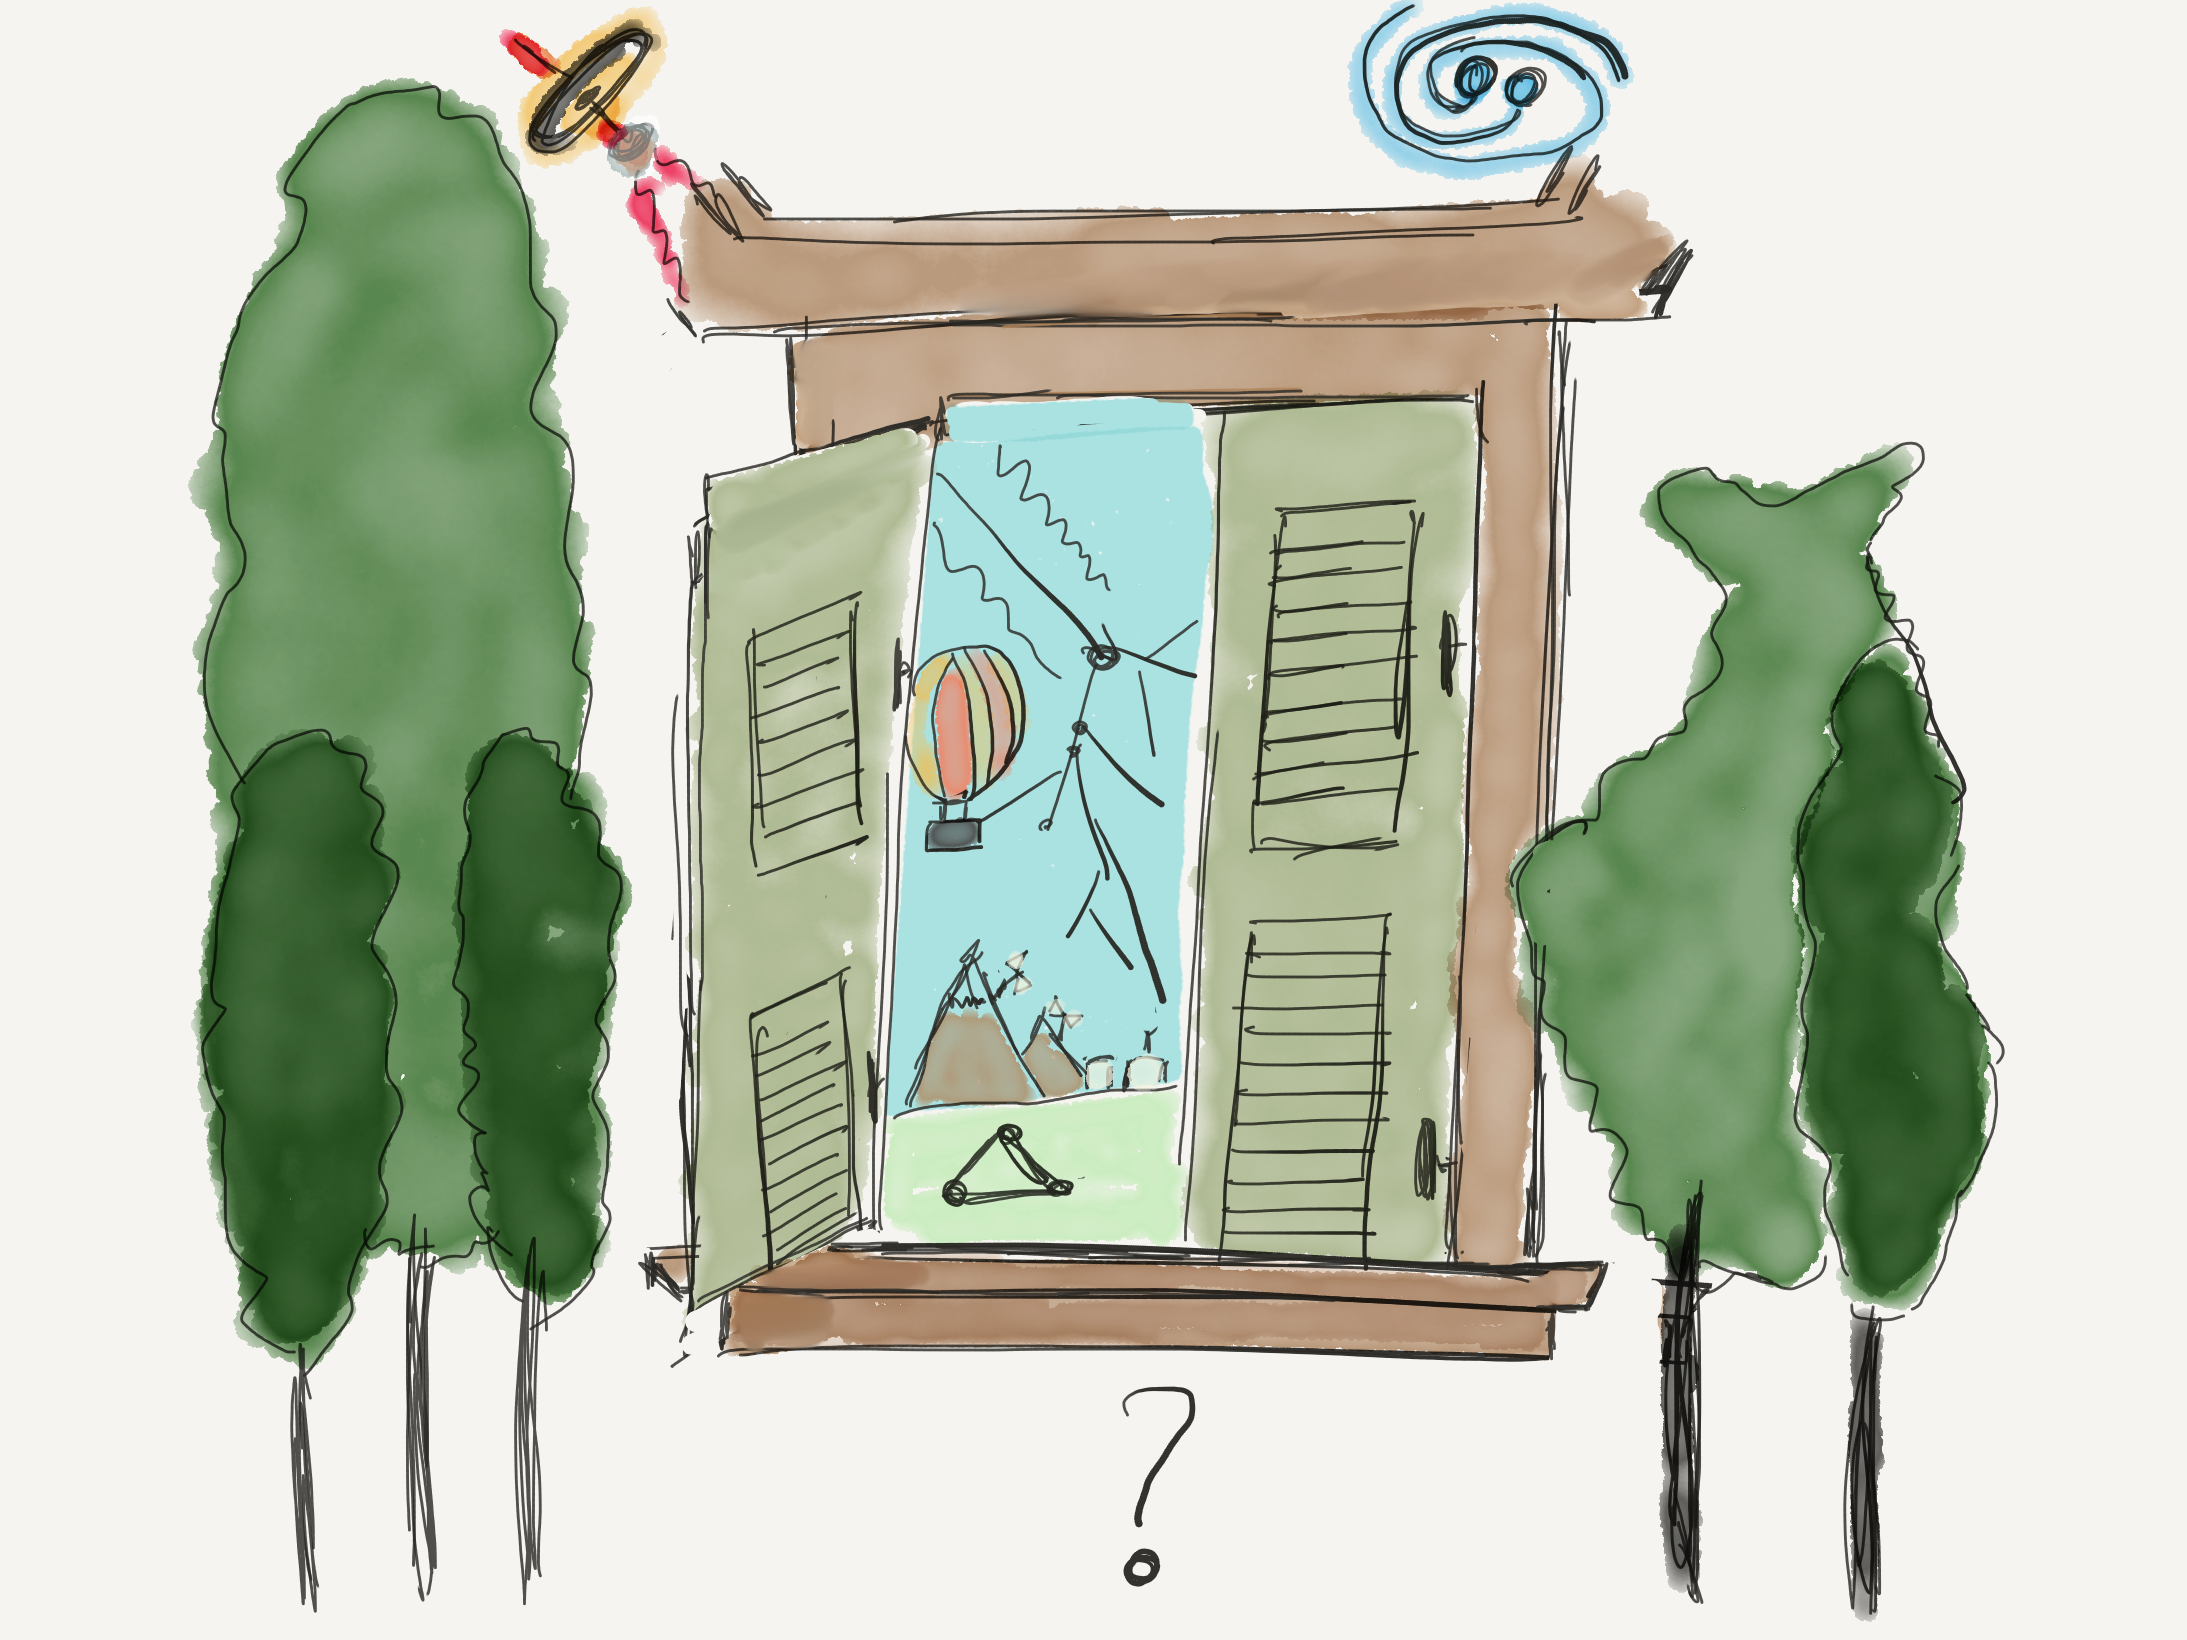
\includegraphics[width=13cm]{thesis_figures/What?.png}
\caption{Window to the inner workings of the Universe is only half opened. (better caption?)}
\label{fig:intro}
\end{figure}
The need to understand how something works or why something is? is ingrained in every human. While attempting to find answers for these questions one either answers them conclusively or finds oneself asking additional questions stemming from the original. One such question which bothered physicists at the beginning of the 20th century and eventually led to the field of \textit{astro-particle physics} was of so-called "atmosphere electricity" or ionization of air. After the pioneering discoveries by Theodor Wulf~\cite{article_Wulf} and Victor Hess~\cite{Hess:1912srp} who found the increase of this ionization rate with altitude and theorized the origin of this radiation to be not earth but something above our atmosphere, the name \textit{cosmic rays} was coined by Robert Millikan who believed these rays were originating from primary photons. This hypothesis was rejected by the measurements done by Jacob Clay~\cite{Clay:1927I,Clay:1928II} in 1927 who observed a latitude dependence of the intensity of cosmic rays concluding this to be a deflection of the primary cosmic-rays(CRs) by the geomagnetic field of the earth which indicated that these rays must be charged particles. After this came the efforts of B. Rossi~\cite{rossi1933eigenschaften}, German group~\cite{schmeiser1938harten} and P. Auger~\cite{RevModPhys.11.288} all independently discovering coincident signals in separated Geiger counters which they explained by the counters being struck by an extensive particle shower triggered by a primary cosmic ray. The phenomenon was named \textit{sciami} by Rossi, \textit{Luftshauer} by the German group and "Auger showers" by Auger and his collaborators. Auger went one step further by further estimating the primary energy of the cosmic ray via his superior setup giving rise to some questions about CRs which are yet unanswered, how are they created and where are they coming from. One of the known sources which is the Sun is too close to explain some other high energy CRs constantly hitting the Earth's atmosphere. Since then the field has only expanded with numerous experiments set up to characterize these cosmic rays. 

The biggest of these experiments which looks for ultra-high energy cosmic rays(UHECRs) exists in 3000 km$^2$ patch of Argentinian pampa just outside Malargue called the Pierre Auger Observatory~\cite{Auger:2015}. It uses a combination of 1660 Water Cherenkov tanks which form the Surface Detector of the observatory and observe the air shower particles arriving at the ground along with Fluorescence Detectors/Telescopes which can look at the development of shower as it travels through the atmosphere. Built primarily to answer the question of the cut-off of the cosmic ray spectrum also known as Greisen–Zatsepin–Kuzmin limit(or GZK cut-off), the observatory has provided immense contributions not only in the field of CRs but also in the fields of Geophysics(elves)~\cite{Mussa_2022}, Dark matter(composition)~\cite{Abreu_2023} and multi-messenger physics(neutrino+photon searches)~\cite{Aab_2019_point,Auger_photons_2022}. Currently, the Surface detector is undergoing an upgrade which will add a scintillator and radio detector on top of the Water Cherenkov tanks further increasing the sensitivity of the Observatory especially to the composition of the cosmic rays.

The non-electrical neutrality of the incoming CRs provides one of the biggest hindrance for finding their sources. This means that CRs do not travel in straight lines from their sources and are affected by the magnetic fields and can also interact with the matter along the way~\cite{bister2024largescaleanisotropyfluxdemagnification, ALLARD201233}. Combined with the fact that the possible sources are light years away from us, without knowing the magnetic fields of the Universe it is very hard to detect the sources of CRs. Ultra High Energy Neutrinos (UHE$\nu_s$) can help in this challenging search for the sources of CRs~\cite{UHEcorrelation_2016}. Being electrically neutral and having a very low interaction cross-section these particles can travel large distances unaffected by the intervening matter and magnetic fields. Several scenarios which are discussed later in section.~\ref{subsubsec:CRmessengers} describe how the UHE$\nu_s$ can be produced by cosmic-rays and can tell us about their sources. Moreover, UHE$\nu_s$ are also interesting as they can also help constrain or explain different production and propagation scenarios for various sources helping us see known astrophysical and cosmogenic objects in a new way. The success of IceCube Neutrino Observatory, a neutrino observatory located in the South Pole,  in detecting the first astrophysical neutrinos and observations of the first steady source NGC 1068~\cite{Icecube_2022} and transient source~\cite{Icecube_txs} have reinvigorated the astro-particle field. The Pierre Auger Observatory has also contributed to the search for UHE$\nu_s$ by trying to detect the Extensive Air SHowers (EASs) that can be induced by them. With its stellar sensitivity at high energy, searches at Pierre Auger Observatory have provided some of the strictest upper limits on the diffuse flux of UHE neutrinos~\cite{Aab_2019_diffuse}. This has already led to constrains on various hypothesized models explaining cosmogenic neutrino production.

The last decade with the successes of LIGO/VIRGO~\cite{PhysRevLett.116.061102} in measuring the first Gravitational waves and IceCube in detecting the first astrophysical neutrinos has also rekindled a field which displays the true spirit of harmony in science and is called multi-messenger astronomy. The aim of the field is to establish a network that can coalesce all the information available through various messengers via which we can see the Universe and maximise the resources and experiments available at Earth. This also allows us to understand the sources better since the observation or non-observation of different messengers can help constrain the mechanisms behind their functioning. The beginning of this field can be traced back to the observation of the first cosmic rays in conjunction with solar flares further cementing the important role Pierre Auger Observatory can play for this field. One of the most important success stories of this field is the August 2017 detection of the neutron star collision~\cite{Abbott_2017} first by the LIGO/VIRGO detector since the Gravitational waves are the fastest messengers and then 1.7s later by the Fermi Gamma ray space telescope and INTEGRAL. 11 hours later already alerted by these two experiments the optical counterpart was detected by multiple telescopes like Las Campanas Observatory and the Hubble Space Telescope. The event was also further seen in Ultraviolet(Neil Gehrels Swift Observatory), X-ray(Chandra X-ray Observatory) and radio(Karl G. Jansky Very Large Array). The non observation of neutrinos by both the IceCube and the Pierre Auger Observatory helped reach the important conclusion about the orientation of the jets which is hypothesized to be off-axis i.e. not pointing directly towards the Earth. Since neutrinos and Gravitational waves are the fastest of the messengers to reach the Earth, alerts issued by IceCube and LIGO/VIRGO are regularly used to follow up the events with other experiments. Subsequent observations of the blazar TXS 0506+056~\cite{TXS_Multi_2018} with IceCube, FERMI-LAT and MAGIC and the observations of neutrinos from the plane of the Milky Way galaxy~\cite{Galactic_plane_nu_2023} have helped establish the continued importance of multi-messenger astronomy.

In this thesis performance of one of the upgrades of the Pierre Auger Observatory done in 2013 is evaluated in the context of neutrino search. This upgrade consisted of introducing new triggers called Time over Threshold deconvulated(ToTd) and Multiple of Positive Steps(MoPS) to reduce the muonic background and effectively decrease the energy threshold for the array. Such triggers can be particularly important in the context of neutrino searches between $60^\circ$-$75^\circ$ since they help in getting a better signal background separation. The effect of these triggers for both the search of a diffused neutrino flux and point like sources of neutrinos is investigated. The thesis also focuses on maximising the previously done neutrino searches in the zenith region $60^\circ$-$75^\circ$ by investigating and updating the analysis presented in~\cite{Aab_2019_diffuse},~\cite{gap_note_2013}.

The thesis is structured as follows, The next chapter~\ref{chap:crnNu} gives the theoretical background for UHE cosmic rays and UHE neutrinos and other important messengers in regard to the Pierre Auger Observatory. It also aims to discuss the various theoretical scenarios involved in their production and propagation. The chapter also aims to summarize the important recent results for these messengers and the various interesting open questions for them. The next chapter~\ref{chap:EAS} describes the phenomenon of Extensive Air showers which is used to indirectly detect both the cosmic rays and neutrinos at the Pierre Auger Observatory. To continue with understanding the detection in a more experimental context the next chapter~\ref{chap:setup} gives a detailed description of the Pierre Auger Observatory. The objective of the chapter is to try to give an exhaustive description of all the tools at the Pierre Auger Observatory necessary to detect neutrinos with a particular focus on the Surface Detector which is of primary concern for the analysis presented in this thesis. A small section is also dedicated to the recently completed AugerPrime upgrade and the exciting potential it offers especially for multi-messenger searches. 

The second part of the thesis is dedicated to the neutrino search in the zenith angular region $60^\circ$-$75^\circ$ (Down-going low, DG$\mathrm{_{low}}$). This part begins with the chapter~\ref{chap:DGL} that gives a description of the neutrino search in the angular range $60^\circ$-$75^\circ$ which is also the primary focus region for this thesis. The chapter is dedicated to provide a complete description of the choices made for the analysis with the proper reasoning. It reports the areas of potential improvements and also communicates the observed improvements to the neutrino search with the new triggers. A new ~\textit{blind} search is performed to look for neutrinos in the data recorded at the Pierre Auger Observatory. The results are summarised at the end of this chapter and due to the non-observance of any neutrino like events, the corresponding limits to the neutrino flux are presented. The Observatory can also detect showers in zenith angle range $75^\circ$-$90^\circ$ (Down-going high, DG$\mathrm{_{high}}$) and up-going showers in the zenith angular region $90^\circ$-$95^\circ$ (Earth-skimming, ES)with the Surface Detector and $90^\circ$-$180^\circ$ (???) with the Fluorescence Detector, but these searches are not performed in this thesis and only their final results are included for comparison and to provide a holistic feel for the neutrino search at Pierre Auger Observatory.

The last part of this thesis presents an example of a neutrino follow-up analysis for point-like sources in chapter~\ref{chap:follow-up}. Due to the non-observance of any neutrinos in the data at the Pierre Auger Observatory an upper limit set by this analysis is also provided for interesting point source neutrino candidates. All the important results are then finally summarised in chapter~\ref{chap:conc} and a short outlook of the future directions for the analysis and the neutrino search at the Pierre Auger Observatory is put forward. The dissertation is completed by three appendices. The first describing the independent work done to compare the various hadronic interaction models for neutrino simulations and the second contains a technical overview of the changes made to implement the $75^\circ$-$90^\circ$ neutrino search within Offline, the software framework of the Pierre Auger Observatory. 

%%% Local Variables:
%%% mode: latex
%%% TeX-master: "mythesis"
%%% End:

% Uncomment the following command to get references per chapter.
% Put it inside the file or change \include to \input if you do not want the references
% on a separate page
% \printbibliography[heading=subbibliography]

%------------------------------------------------------------------------------
% Use biblatex for the bibliography
% Add bibliography to Table of Contents
% Comment out this command if your references are printed for each chapter.
\printbibliography[heading=bibintoc]

%------------------------------------------------------------------------------
% Include the following lines and comment out \printbibliography if
% you use BiBTeX for the bibliography.
% If you use biblatex package the files should be specified in the preamble.
% \KOMAoptions{toc=bibliography}
% {\raggedright
%   \bibliographystyle{../refs/atlasBibStyleWithTitle.bst}
%   % \bibliographystyle{unsrt}
%   \bibliography{./thesis_refs,../refs/standard_refs-bibtex}
% }

%------------------------------------------------------------------------------
\appendix
% \part*{Appendix}
% Add your appendices here - don't forget to also add them to \includeonly above
\include{thesis_appendix}
% \printbibliography[heading=subbibliography]

%------------------------------------------------------------------------------
% Declare lists of figures and tables and acknowledgements as backmatter
% Chapter/section numbers are turned off
\backmatter

\listoffigures
\listoftables

%------------------------------------------------------------------------------
% Print the glossary and list of acronyms
% \printglossaries

%------------------------------------------------------------------------------
% You could instead add your acknowledgements here - don't forget to
% also add them to \includeonly above
% %------------------------------------------------------------------------------
\chapter*{Acknowledgements}
\label{sec:ack}
%------------------------------------------------------------------------------
Even though this thesis has my name on the front a number of people were involved in shaping its final form both in person and in spirit.

First and foremost I would like to thank my late grandfather Shanti Sarup Sehgal and grandmother Kusum Sehgal. Their constant motivation and belief in my abilities has and will always inspire me to achieve more.

I am very grateful to Professor Bernhard Ketzer for giving me an opportunity to write my thesis in his group. In spite of my many shortcomings and failures he has always been patient and supportive during the entire time and has been a role model I look up to. I would also like to thank Professor Jochen Dingfelder. I have always admired your lectures and am thankful that you agreed to be my second supervisor.

A special thanks to PhD students Michael Hösgen and Martin Hoffmann for helping with the editing of this thesis. Thank you to Michael for always answering my various questions and solving my problems without which this thesis would have never been completed. A big thanks to the whole AG Ketzer group for both the academic and moral support.

I am grateful to my father Ravi Sehgal, my mother Rajni Sehgal and my brother Sambhav for all the sacrifices they have made. Without their constant support studying at Bonn would have just remained a pipe dream. Lastly, I am thankful to the wonderful set of friends I am lucky to have. Thank you Svenja ,Georgios and Amitayus for the countless Mensa lunches which helped me remain sane throughout the thesis.

%%% Local Variables:
%%% mode: latex
%%% TeX-master: "../mythesis"
%%% End:


%------------------------------------------------------------------------------
% CV needed when you submit your PhD thesis
% \definecolor{lightgray}{gray}{0.8}
\newcolumntype{L}{>{\raggedleft}p{0.15\textwidth}}
\newcolumntype{R}{p{0.8\textwidth}}
\newcommand\VRule{\color{lightgray}\vrule width 0.5pt}

\thispagestyle{empty}
\section*{Curriculum Vitae}

\subsection*{Personal Details}

\begin{tabular}{L!{\VRule}R}
Name & Johann Schmidt \\
Date of Birth &  \\
Email & abc@physik.uni-def.de \\
Family status & Single
\end{tabular}

\subsection*{Education}

\begin{tabular}{L!{\VRule}R}
1997--2003 & Abitur, ABC Secondary School, Hamburg, Germany\\
2004--2007 & BSc in Physics, Rheinische Friedrich-Wilhelms-Universität, Bonn, Germany.\\
2006 & CERN Summer Student, Geneva, Switzerland. \\
2007--2009 &  MSc in Physics Rheinische Friedrich-Wilhelms-Universität, Bonn, Germany. \\
2009--2012 &  PhD in Physics, Rheinische Friedrich-Wilhelms-Universität, Bonn, Germany. \\
2012 & Advanced Data Analysis School, Frankfurt, Germany.
\end{tabular}

\subsection*{Professional Experience}

\begin{tabular}{L!{\VRule}R}
2004 & Summer Student at CERN, Geneva, Switzerland. \\
2007--2012 & Doctoral work at the University of Bonn, Germany. \\
2008--2009 & Fieldwork at CERN, Geneva, Switzerland.\\
2011 & Talk at the Advanced Physics Conference, Timbucto
\end{tabular}

\subsection*{Languages}
\begin{tabular}{L!{\VRule}R}
German & Mother tongue \\
English & Fluent \\
Russian & Basic
\end{tabular}


\end{document}

%%% Local Variables:
%%% mode: latex
%%% TeX-master: t
%%% End:
